\documentclass[12pt,a4paper]{article}
\usepackage[utf8]{inputenc}
\usepackage[danish]{babel}
\usepackage{amsmath}
\usepackage{amsfonts}
\usepackage{amssymb}
\usepackage{graphicx}
\usepackage[left=2cm,right=2cm,top=2cm,bottom=2cm]{geometry}


\usepackage{titlepic}
\usepackage{enumerate}
\usepackage{enumitem}
\usepackage{float}
\usepackage{pdfpages}
\usepackage[colorlinks = true,
            linkcolor = blue,
            urlcolor  = blue,
            citecolor = blue,
            anchorcolor = blue]{hyperref}
\usepackage[explicit]{titlesec}
\usepackage{pstricks}
\usepackage[amsmath,thmmarks]{ntheorem} %pakke til at lave sætningsenvorinmets (kan ikke loades sammen med amsthm)
\usepackage{color}
\usepackage{tikz}

%opretter environmets til sætningsstrukturen 
\theorembodyfont{\normalfont}

	
	%sætnings environment	
	\newtheorem{thm}{Sætning}

	\theoremstyle{break}	
	%opgave environment	
	\newtheorem{opg}{Opgave}	

	%Korrolar environment
	\newtheorem{korollar}[thm]{Korollar}	
	
	%Lemma environment	
	\newtheorem{lemma}[thm]{Lemma}
	
	\theoremsymbol{\ensuremath{\circ}}	
	
	%definition environment	
	\newtheorem{definition}[thm]{Definition}
	
	%eksempel environment	
	\newtheorem{eksempel}[thm]{Eksempel}
	
	
	
	%Bevis environment
	\theoremstyle{nonumberplain}
	\theoremheaderfont{%
	\normalfont\itshape}
	\theorembodyfont{\normalfont}
	\theoremsymbol{\ensuremath{\square}}
	\theoremseparator{.}
	
	\newtheorem{proof}{Bevis}
	\newtheorem{los}{Løsning}
	






\setlength\parindent{0pt}

%\titleformat{\section}{\Large\bfseries}{}{0pt}{#1}
%\titleformat{\subsection}{\large\bfseries}{}{0pt}{#1}


%nye komandoer
\newcommand{\mR}{\mathbb{R}}
\newcommand{\mZ}{\mathbb{Z}}
\newcommand{\mN}{\mathbb{N}}
\newcommand{\mQ}{\mathbb{Q}}
\newcommand{\mC}{\mathbb{C}}
\newcommand{\hs}{\hspace{2mm}}
\newcommand{\Hs}{\hspace{4mm}}
\newcommand{\pipe}{\hs | \hs}
\newcommand{\lp}{\left(}
\newcommand{\rp}{\right)}
\newcommand{\vect}[1]{\underline{#1}}
\newcommand{\matr}[1]{\underline{\underline{#1}}}
\newcommand{\cnum}[1]{\raisebox{.5pt}{\textcircled{\raisebox{-.9pt} {#1}}}}




\author{Mikkel B. Goldschmidt\\ 3r, Nørre Gymnasium \\ AT: Matematik og fysik}
\title{AT6 - Menneskets forhold til naturen \\ Deterministisk kaos}
\date{\today}


\usepackage{csquotes}

\begin{document}
\includepdf{forside}

\maketitle

\section{Indledning}
I 1814 skrev Laplace om en dæmon, der kendte til altings placering, fart, temperatur og alle andre fysiske og kemiske egenskaber ved verden.
Laplace argumentere for, at denne dæmon måtte kende alt fremtid og alt fortid, hvis den ellers var i stand til at kigge på alt dette data. 
Han skrev om sin idé om at en person med alt denne viden, måtte kunne beskrive verden i en matematisk ligning. 
Ultimativt skulle det være drømmen for naturvidenskaben: At vide nok til at kunne beskrive verden perfekt - og dermed vide alt.

For 50 år siden ødelagde matematikeren og metrologen Edward Lorenz dog denne drøm. 
Han havde opsat et differentialligningssystem, der kunne beskrive vejret i fremtiden ud fra en række parametre. 
Da han ikke kunne løse modellen analytisk, brugte han en numerisk løsning med en computer. 
Han prøvede dog på et tidspunkt at regne ud, hvordan vejret ville se ud om et år. 
Først regnede han et år frem i modellen og fandt et resultat. 
Han fandt dog ved et tilfælde ud af, at dette gav et fuldstændigt andet resultat end ved først at regne et halvt år frem og, derefter  regne endnu et halvt år frem, ved at bruge de tal som modellen gav. 
Årsagen til dette skulle findes i, at hans model afrundede til betydende cifre. 
Det, at nogle cifre var blevet tabt, gav altså et helt andet resultat. 
Denne relativ lille ændring i input gav altså ikke en relativ lille ændring i output. 
Han navngav dette fænomen \textit{deterministisk kaos}.
Det skulle vise sig, at deterministisk kaos var et argument for, at Laplace dæmon aldrig ville kunne eksistere i virkeligheden.

\section{Problemformulering}
I hvor høj en grad begrænser en kaotisk verden vores beskrivelse af naturen?

\begin{itemize}
\item Hvad forstås ved deterministisk kaos, og hvornår opstår det?
\item Hvordan kommer deterministisk kaos til udtryk i trelegemeproblemet?
\item Gør deterministisk kaos vores normale naturvidenskabelige praksis ubrugelig?
\item Hvordan passer det deterministiske kaos, med den menneskelige intuition om hvordan verden opfører sig?
\end{itemize}

\section{Behandling af underspørgsmål}

\subsection{Kaos}
Lorenz definerer kaos på følgende måde:
\begin{displayquote}
\textit{When the present determines the future, but the approximate present does not approximately determain the future.}

- Edward Lorenz, nedskrevet på et stykke papir på University of Maryland i 2005\footnote{\url{http://mpe2013.org/2013/03/17/chaos-in-an-atmosphere-hanging-on-a-wall/}}

\end{displayquote}
	
Han fandt adskillige differentialligningssystemer hvor kaos opstår.
Kaos er derefter blevet opdaget i mange systemer, der beskriver naturen. 

Til besvarelsen af dette spørgsmål har jeg refereret til andre der har brugt naturvidenskabelig metode. 
Den vej jeg har arbejdet i hele denne proces, har i virkeligheden været en kopi af den måde, som Lorenz arbejdede på, da han opdagede kaos som fænomen.

\subsection{Trelegemeproblemet}
I sin bog, Principia, skrev Newton blandt andet om sine gravitationslove. 
Han overvejede ud fra disse love hvordan forskellige objekter ville opføre sig i forhold til hinanden. 
Blandt andet finder han pæne stedfunktioner for to legemer der påvirker hinanden med gravitationskræfter. 
Det lykkes ham til gengæld ikke at gør det samme med tre legemer, og han opstiller det derfor som et problem som andre kan arbejde videre med. 

Det har senere vist sig at grunden til at det var så svært for Newton, var at trelegemeproblemet er et system hvor der opstår kaos. 

Dette er noget jeg har læst, men jeg besluttede mig for at efterprøve det. 
Jeg brugte derfor fysikken til at opstille et differentialligningsystem med 3 legemer, der påvirker hinanden med gravitationskræfter. 


$$\vec{a_1} = \vec{s_1}'' = G \cdot \dfrac{m_2 \cdot (\vec{s_2} - \vec{s_1})}{dist(\vec{s_1}, \vec{s_2})^3} + G \cdot \dfrac{m_3 \cdot (\vec{s_3} - \vec{s_1})}{dist(\vec{s_1}, \vec{s_3})^3}
$$

$$\vec{a_2} =  \vec{s_2}'' = G \cdot \dfrac{m_1 \cdot (\vec{s_1} - \vec{s_2})}{dist(\vec{s_2}, \vec{s_1})^3} + G \cdot \dfrac{m_3 \cdot (\vec{s_3} - \vec{s_2})}{dist(\vec{s_2}, \vec{s_3})^3}$$

$$\vec{a_3} = \vec{s_3}'' = G \cdot \dfrac{m_1 \cdot (\vec{s_1} - \vec{s_3})}{dist(\vec{s_3}, \vec{s_1})^3} + G \cdot \dfrac{m_2 \cdot (\vec{s_2} - \vec{s_3})}{dist(\vec{s_3}, \vec{s_2})^3}$$

Her beskriver $\vec{s_i}$ en stedvektor for legeme $i$, 
$\vec{a_i}$ en accelerationsvektor for legeme $i$, 
$m_i$ en masse legeme $i$,
$dist(v,u)$ beskriver den numeriske afstand mellem to vektorer $v$ og $u$, og
$G$ er den universelle gravitationskonstant.

Dette differentialligningssystem er et koblet, andenordens og ikke-lineært system, og vi har derfor ikke metoder til at finde generelle løsninger i det indenfor pensum.

Jeg har derfor løst problemet ved at løse systemet numerisk. 
For at gøre det simpelt har jeg gjort brug af Eulers metode.
Systemet er lavet i 2D for at gøre illustrationen mere overskuelig.

Jeg har opsat nogle startbetingelser med sted- og hastighedsvektorer for hvert legeme.
Fra disse startbetingelser har jeg så kunnet regne en accelerationsvektor. 
Ved at steppe et stykke i tid har jeg da fra accelerationen kunne beregne en ny hastighed og derfra en ny stedvektor.

Jeg kører da to systemer oveni hinanden uafhængigt af hinanden (det ene vist med hvidt, det andet med rødt). 
De to systemer har næsten samme startbetingelser, jeg har bare ændret startstedvektoren for en af legemerne med $0.0000001$ pixels.
 
Denne algoritme har jeg da implementeret i Javascript, hvor jeg har brugt pakken P5 til at tegne stedvektorerne som cirkler.
I bilaget ses min sourcekode sammen med et link til GitHub, hvor jeg løbende opdaterer koden op til eksamen, hvis jeg finder eventuelle småfejl eller der er noget æstetisk, jeg vil ændre på. 

Jeg har da kørt simulationen.
Til at starte med kan man kun se det ene system, da det bliver printet oveni det andet, men efter ca. 30 sekunder (med de startbetingelser jeg har opsat) bliver kaos tydeligt. 
De to systemer begynder at opføre sig helt forskelligt. 
Dette viser klart hvordan en en approksimation af det røde systems startbetingelser, ikke giver en approksimation af det røde systems betingelser efter 30 sekunder. 



Denne opdagelse er ret central, for det udelukker faktisk at vi nogensinde vil kunne forudsige naturen længere ud i fremtiden, da der i langt de fleste systemer er minimum tre legemer (det kan enten være planeter, elektroner eller luftmolekyler - problemet opstår alle steder). 
Og denne simulation viser os netop, at kaos opstår i systemer med 3 legemer.

Ved at indse at der opstår kaos i alle systemer med minimum tre legemer, bliver vi faktisk også nødt til at indse, at naturen er umulig at forudsige, så længe vi ikke kan måle og regne uendelig præcist.

Til besvarelsen af dette delspørgsmål har jeg brugt fysikken til at beskrive naturen med en matematisk model. 
Herfra har jeg da kunnet lade matematikken tage over, og ved brug af numerisk metode kunne finde en løsning i modellen. 
Fysikken kan altså beskrive naturen hvor matematikken kan se de logiske konsekvenser af beskrivelsen.

\subsection{Videnskabelig praksis i en kaotisk verden}
Når vi laver naturvidenskab, er det ofte vores mål, at få opstillet regler der er så generelle, at de kan bruges til at forudsige verden med. 
Med tilstrækkelige oplysninger, mener vi at kunne give en nogenlunde beskrivelse af hvad der kommer til at ske med verden lige om lidt.
Eksempelvis er de fleste stærkt overbeviste om at når du giver slip på en blyant, så falder den til gulvet. 
Lidt forudsigelighed har vi altså i verden. 
En kritiker kunne så spørge hvorfor kaos overhovedet er relevant, når nu vi kan forudsige nogle ting. 
Selvom vi kan lave forudsigelser om verden på kort sigt, så opstår der problemer på længere sigt. 
Vi oplever det dagligt efter nyhederne om aftenen, når metrologen går på. 
Metrologerne lever af at forudsige verden et stykke frem i tiden, men alle ved også godt, at de ofte tager fejl, og at man aldrig kan regne med dem mere en et par dage frem. 
Det er ikke fordi vores metrologerne er inkompetente, de arbejder bare med et kaotisk system - naturen.
Det er klart nemt for dem at sige hvordan vejret ser ud om en time, og de vil kunne sige dem med forholdsvist stor nøjagtighed. 
Men spørger man dem om hvordan vejret ser ud om præcis 4 måneder, ved de godt at de ikke har en chance. 
De kan nemlig kun regne på approksimationer af virkeligheden, og i kaotiske systemer, giver disse ikke en approksimation af virkeligheden.

Vi må derfor indse at naturvidenskaben aldrig kommer til at forudsige verden længere frem i tiden. 

Besvarelsen af dette spørgsmål bygger mest på opdagelserne i forrige spørgsmål. 
Jeg kigger altså på de konsekvenser opdagelserne i sidste spørgsmål har, og jeg bruger derfor ikke fagene direkte her. 

\subsection{Den menneskelige intuition om en kaotisk verden}
Laplace dæmon, som beskrevet i indledningen, beskriver nok den intuition som mange mennesker har, når de starter på at lave naturvidenskab, og den intuition der har været almindelig blandt fysikere indtil opdagelsen af kvantemekanikken - nemlig at verden er deterministisk.

Med deterministisk kaos må vi indse, at dette ikke er muligt med determinismen i praksis. 
Vi ville kun kunne det, hvis vi kunne måle uendelig præcist og regne lige så præcist, hvilket oplagt ikke er muligt.

Vi kan dog godt lave approksimationer af virkeligheden over kortere tid der er forholdsvist præcise. 

Dermed er naturvidenskaben stadig brugbar, men vi er ikke i stand til at forudsige, hvordan naturen vil opføre sig præcist.

\section{Fagenes metoder}
Fysik og matematik er to fag der spiller godt sammen, og i langt det meste fysik er matematik uundgåeligt. 
Jeg har i denne opgave ikke brugt den naturvidenskabelige metode direkte, men jeg har i stedet bygget på andre, der har gjort det. 
Havde jeg skullet gøre det hele fra bunden, ville jeg blive nødt til at have bekræftet Newtons gravitationslove ved brug af eksperimenter. 

Matematikken har jeg til gengæld brugt meget klassisk. 
Jeg har bare kigget på hvilke logiske konsekvenser et opstillet system har. 
Det er dog værd at bemærke, at jeg har hevet teknikker ind fra datalogi, som af de fleste betragtes som et sidefag til matematikken. 

\section{Konklusion}
Deterministisk kaos er når bare små afvigelser i et systems startbetingelser, har store indflydelser på systemet over længere tid.
Fænomenet opstår mange stedet, specielt vigtigt er det at det opstår mange stedet i naturen. 
Et sted hvor det kommer til udtryk i Newtons trelegemeproblem, hvor man kan se kaos direkte i et system meget hurtigt.

Det deterministiske kaos gør ikke vores naturvidenskab ubrugelig, men vi må indse at der er begrænsninger for hvor meget vi kan forudsige, specielt hvor langt ud i fremtiden vi kan forudsige ting. 
Dette passer ikke umiddelbart med den intuition som man har haft for naturvidenskaben meget længe. 
Dog kan vi stadig bruge den naturvidenskab vi har, da de små fejlmålinger ikke har den store indflydelse på kort sigt. 
Altså er den eneste intuition vi må give afkald på, at vi kan forudsige fremtiden helt præcist med tilstrækkelige oplysninger.

\section{Perspektivering}
\subsection{Studierapport}
Dette forløb minder en del om mit sidste AT-forløb i den måde matematikken er blevet brugt på. 
Da jeg arbejdede med epidemier, brugte jeg også numeriske løsninger af differentialligninger til at løse et problem. 

\subsection{Perspektivering}
Med kaosteori i baghånden får de meget små tilfældigheder, der præsenteres i kvantemekanikken, en helt anden betydning. 
Det at meget små hændelser, som eksempelvis et henfald af en radioaktiv kerne, ved vi lige pludselig, kan have meget vidtrækkende konsekvenser over tid. 
Filosofisk får de kvantemekanikken altså en helt anden slagkraft, når den kombineres med kaosteori.

\pagebreak
\section{Kilder}
\begin{itemize}
	\item Chaos in an Atmosphere Hanging on a Wall, Christopher M. Danforth, Ph.D., University of Vermont\\
	\url{http://mpe2013.org/2013/03/17/chaos-in-an-atmosphere-hanging-on-a-wall/}
	
	\item Wikipedia: Edward Norton Lorenz\\
	\url{https://en.wikipedia.org/wiki/Edward_Norton_Lorenz}
	
	\item Wikipedia: Chaos Theory\\
	\url{https://en.wikipedia.org/wiki/Chaos_theory}
	
	\item Eulers metode fra Matematiksider.dk\\
	\url{http://www.matematiksider.dk/projekter/eulers_metode.pdf}
	
\end{itemize}

\section{Bilag}
\begin{itemize}
	\item Sourcekode til simulation. Link til GitHub:\\ \url{https://github.com/mikkelbjoern/threeBodyProblem}
	\item Forsimplet flowchart over algoritmen brugt i min simulation
	
\end{itemize}

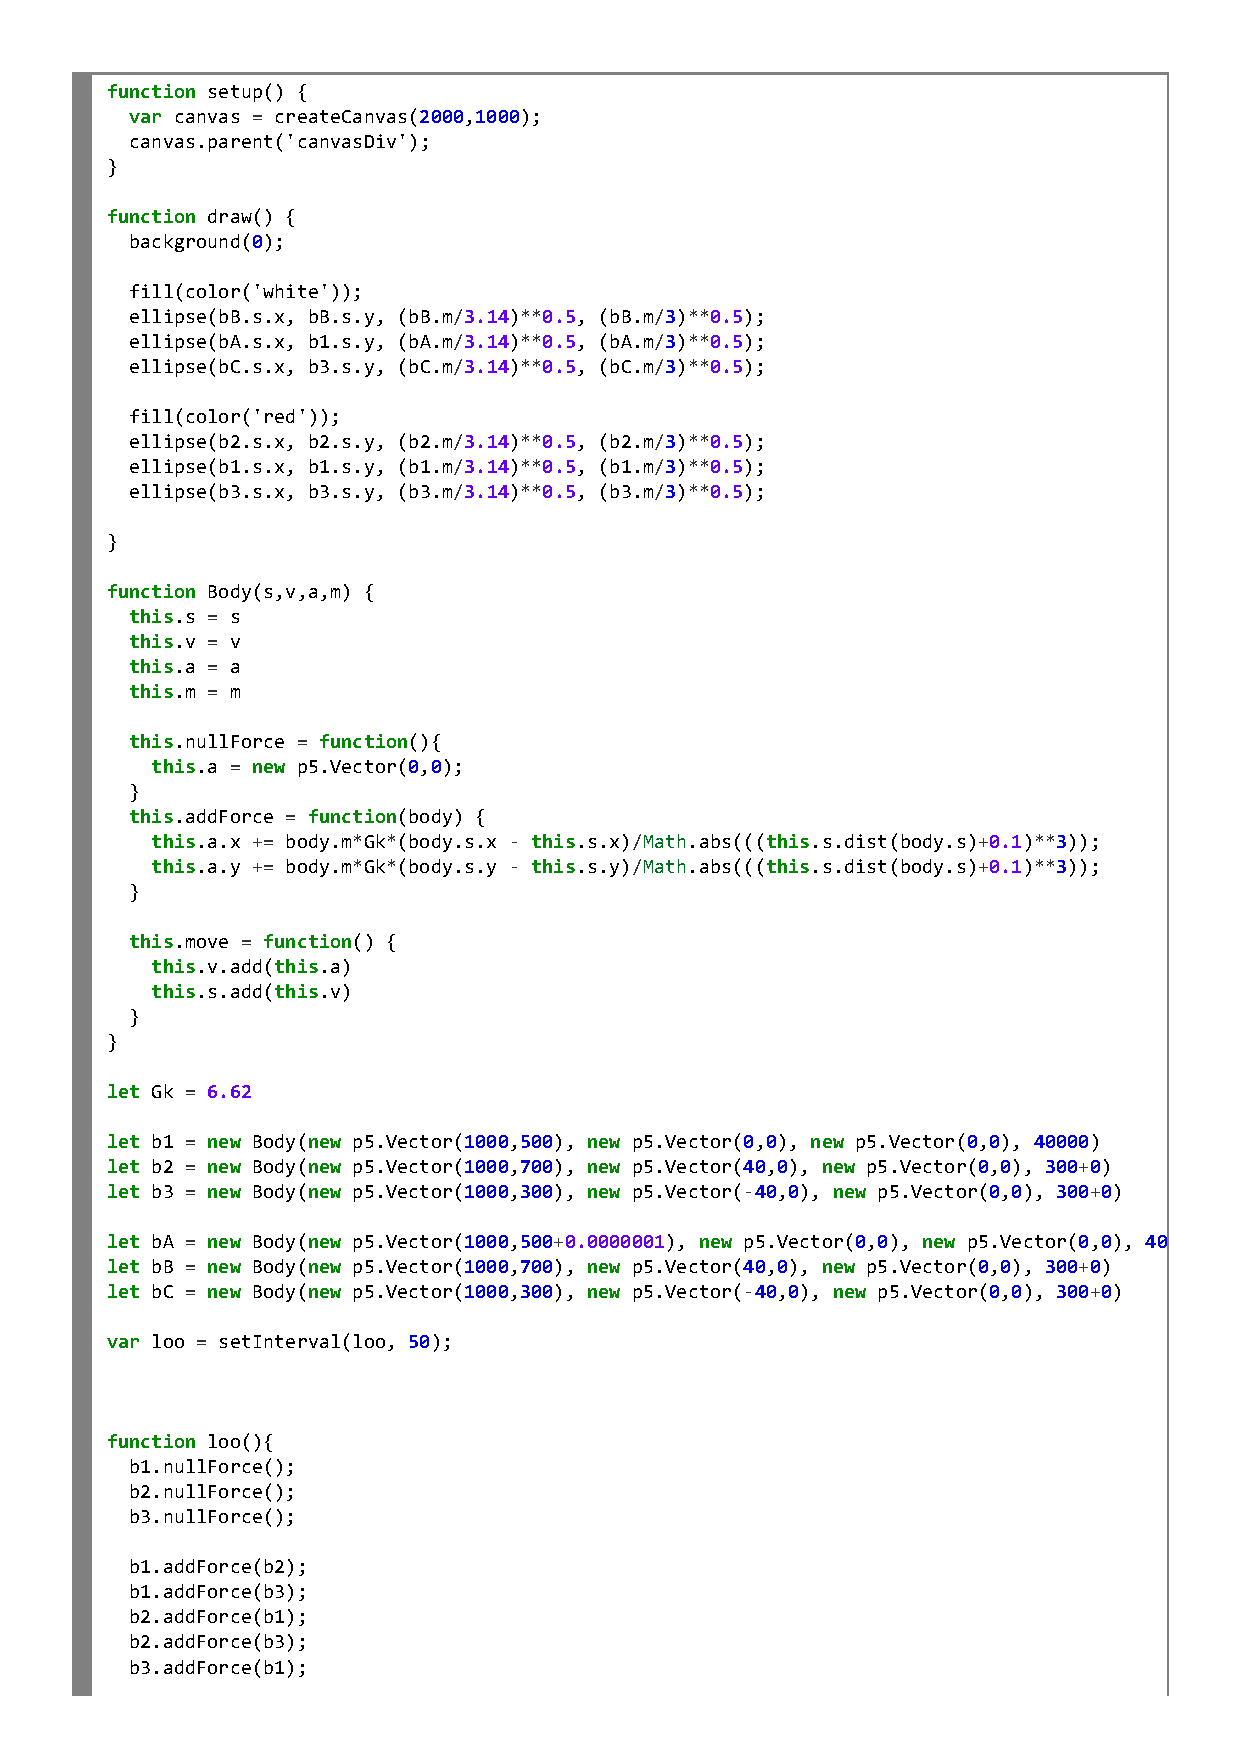
\includepdf[pages=-]{prettyCode.pdf}

\subsection*{Forsimplet flowchart over algoritmen brugt i min simulation}

\begin{figure}[h]
\begin{center}
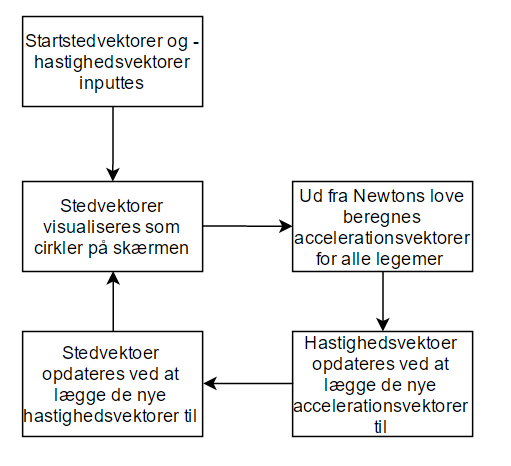
\includegraphics[scale=1]{algorithm}
\end{center}
\end{figure}

\textit{Bemærk:} Dette flowchart er forsimplet.
Når sted- og hastighedsvektorer beregnes, er der taget højde for, at der skal ganges en tidsforskel på. 
De præcise udregninger er ikke skrevet på for at gøre algoritmen simpel at forstå.
\end{document}